\documentclass[french, toc]{../cs-classes/cs-classes}

\graphicspath{{./images}}

\title{Systèmes d'exploitation}
\author{Timothy Bourke, Marc Pouzet\\ Notes par Antoine Groudiev}
\date{Version du \today}

\begin{document}
\newpage
\section*{Introduction}
Ce document est l'ensemble non officiel des notes du cours \emph{Systèmes d'exploitation} du Département Informatique de l'ENS Ulm. Elles sont librement inspirées des notes de cours sous forme de présentation rédigées par Timothy Bourke et Marc Pouzet.

\section{Micro-noyau}
Commençons ce cours par la programmation d'un micro-noyau fortement simplifié, implémenté en OCaml. Notre objectif sera de retenir l'essentiel d'un noyau de système classique, en exécutant le moins de fonctions possibles en mode super-utilisateur\footnote{Les fonctions exécutées en mode "super-utilisateur" ont un accès non protégé aux ressources.}.

\subsection{Description générale d'un micro-noyau}
Un micro-noyau contient une ou plusieurs \emph{applications}, comme un système de fichier ou un driver de disque.

Les principales fonctionnalités d'un micro-noyau sont de gérer les processus, la communication entre eux, et la mémoire virtuelle. Il doit être capable de créer, arrêter, ordonner les processus en fonction de leur priorité.

On se donne les caractéristiques suivantes pour l'architecture machine:
\begin{itemize}
    \item elle est capable d'exécuter un seul processus à la fois
    \item elle possède cinq registres, de \texttt{r0} à \texttt{r4}
\end{itemize}

\subsection{Appels système}
Le micro-noyau doit être capable de réagir à deux types d'évènements:
\begin{itemize}
    \item l'interruption d'un compteur de temps (\texttt{timer})
    \item des interruptions logicielles (\texttt{system trap} ou \texttt{software interrupt})
\end{itemize}
Les processus de l'utilisateur peuvent changer le contenu des registres et générer des appels système arbitraires. Quand un appel système est déclenché, le micro-noyau lit le contenu des registres pour déterminer l’appel effectué et les arguments de cet appel. Il réagit en effectuant l’appel (par exemple, la mise à jour de l’état du système) et en plaçant les valeurs de retour dans les registres.

On définit les codes d'appels systèmes suivants:
\begin{figure}[!ht]
    \centering
    \begin{tabular}{c c}
        Registre \texttt{r0} & Appel système \\
        \hline
        \texttt{0} & \texttt{new\_channel} \\
        \texttt{1} & \texttt{send} \\
        \texttt{2} & \texttt{receive} \\
        \texttt{3} & \texttt{fork} \\
        \texttt{4} & \texttt{exit} \\
        \texttt{5} & \texttt{wait} \\
    \end{tabular}
\end{figure}
En cas d'appel système invalide (pour une valeur de \texttt{r0} non renseignée dans le tableau), le noyau n'exécute aucun code et place la valeur -1 dans \texttt{r0}.

\subsection{Constantes et types OCaml}
On définit les constantes et type OCaml suivant pour représenter notre micro-noyau:
\begin{minted}{ocaml}
let max_time_slices = 5 (* 0 <= t < max_time_slices *)
let max_priority = 15 (* 0 <= p <= max_priority *)
let num_processes = 32
let num_channels = 128
let num_registers = 5

type pid = int (* process id *)
type chanid = int (* channel id *)
type value = int (* values transmitted on channels *)
type interrupt = int (* software interrupt *)
type priority = int (* priority of a process *)

type registers = {
    r0 : int;
    r1 : int;
    r2 : int;
    r3 : int;
    r4 : int; 
}

let get_registers { registers } = {
  r0 = registers.(0); r1 = registers.(1);
  r2 = registers.(2); r3 = registers.(3);
  r4 = registers.(4); }
(* the set of processes ordered by priority *)

let set_registers { registers } { r0; r1; r2; r3; r4 } =
  registers.(0) <- r0; 
  registers.(1) <- r1;
  registers.(2) <- r2; 
  registers.(3) <- r3;
  registers.(4) <- r4
\end{minted}

\noindent On définit ensuite un processus à l'aide du type suivant:

\begin{minted}{ocaml}
type process_state =
    | Free (* non allocated process *)
    | BlockedWriting of chanid
    | BlockedReading of chanid list
    | Waiting
    | Runnable
    | Zombie

type process = {
    mutable parent_id : pid;
    mutable state : process_state;
    mutable slices_left : int;
    saved_context : int array;
}
\end{minted}

\noindent Les états des processus sont décrits par le diagramme ci-dessous:

% TODO: diagramme

\noindent On définit par ailleurs un état du noyau à l'aide du type \texttt{state} suivant:
\begin{minted}{ocaml}
type channel_state =
    | Unused (* non allocated channel *)
    | Sender of pid * priority * value
    | Receivers of (pid * priority) list

type state = {              (* kernel state *)
    mutable curr_pid   : pid; (* process id of the running process *)
    mutable curr_prio  : priority; (* its priority *)
    registers  : int array;        (* its registers *)
    processes  : process array;       (* the set of processes *)
    channels   : channel_state array; (* the set of channels *)
    runqueues  : pid list array;
}

let get_current { curr_pid = c } = c
\end{minted}

\noindent Finalement, on définit un évènement, qui peut être soit un \texttt{timer}, soit un appel système:
\begin{minted}{ocaml}
type event = | Timer | SysCall

type syscall =
    | Send of chanid * value
    | Recv of chanid list
    | Fork of priority * value * value * value
    | Wait
    | Exit
    | NewChannel
    | Invalid
\end{minted}

\subsection{Détermination de l'appel système}
Ajoutons une fonction \texttt{decode: state -> syscall} qui décode la valeur des registres et détermine l'appel système.
\begin{minted}{ocaml}
let decode { registers } =
match registers.(0) with
| 0 -> NewChannel
| 1 -> Send (registers.(1), registers.(2))
| 2 -> Recv [registers.(1);
             registers.(2);
             registers.(3);
             registers.(4)]
| 3 -> Fork (registers.(1), registers.(2),
             registers.(3), registers.(4))
| 4 -> Exit
| 5 -> Wait
| _ -> Invalid
\end{minted}

\subsection{Appel système \texttt{fork}}
\paragraph*{Description}
L'appel système \texttt{fork} crée un nouveau processus fils. Chaque processus est associé à une priorité comprise entre 0 (la plus basse) et 15 (la plus haute). Le registre \texttt{r1} spécifie la priorité du processus créé. 

Si la priorité donnée est strictement plus grande que la priorité du processus qui crée le processus fils, l’appel système se termine sans créer de processus et en plaçant 0 dans \texttt{r0}. Concrètement, un processus ne peut pas engendrer un processus de priorité plus élevée que la sienne. 

Si la priorité est valide et qu’un nouveau processus peut être créé, \texttt{r0} reçoit la valeur 1 et \texttt{r1} reçoit le numéro du processus créé. Si un nouveau processus ne peut pas être créé, \texttt{r0} reçoit la valeur 0. Ceci arrive en particulier lorsque le nombre maximum de processus pouvant être créés est égal à \texttt{num\_processes}.

Dans le processus fils créé, \texttt{r0} est initialisé à 1, \texttt{r1} est initialisé au numéro de processus du père (qui a fait l’appel à \texttt{fork}), et les autres registres (\texttt{r2}, \texttt{r3} et \texttt{r4}) sont copiés du processus parent.

\paragraph*{Implémentation} On implémente \texttt{fork} sous la forme d'une fonction de type
\begin{center}
    \texttt{fork: state -> int -> int -> int -> int -> unit}
\end{center}
qui sera appelée sous la forme
\begin{center}
    \texttt{fork state nprio d0 d1 d2}
\end{center}
où \texttt{state} est l'état du système, \texttt{nprio} est la priorité à donner au processus fils, \texttt{d0}, \texttt{d1} et \texttt{d2} sont les valeurs à passer au fils pour initialiser ses trois derniers registres.

\begin{minted}{ocaml}
let fork { curr_pid; curr_prio; registers; processes; runqueues } nprio d0 d1 d2 =
    let rec new_proc i =
        if i >= num_processes then None
        else if processes.(i).state = Free then
            let np = processes.(i) in
            np.parent_id <- curr_pid;
            np.state <- Runnable;
            np.slices_left <- max_time_slices;
            np.saved_context.(0) <- 2;
            np.saved_context.(1) <- curr_pid;
            np.saved_context.(2) <- d0;
            np.saved_context.(3) <- d1;
            np.saved_context.(4) <- d2;
            Some i
        else new_proc (i + 1)
    in
    match new_proc 0 with
    | None -> registers.(0) <- 0
    | Some npid -> begin
            registers.(0) <- 1;
            registers.(1) <- npid;
            runqueues.(nprio) <- runqueues.(nprio) @ [npid]
        end
\end{minted}

\subsection{Appel système \texttt{exit}}
\paragraph*{Description} 
L'appel système \texttt{exit} termine l'exécution du processus l'exécutant. Son argument, la valeur de retour de l'appel, est placé dans le registre \texttt{r1}.

Après appel à \texttt{exit}, le processus entre dans l'état \texttt{Zombie}, et ce jusqu'à l'exécution de l'appel système \texttt{wait} qui récupèrera la valeur de retour.

Si le processus terminé avait des fils, ils deviennent \emph{orphelins}. L'identifiant de leur père devient alors le processus 1, appelé \texttt{init}.

\paragraph*{Implémentation} On implémente \texttt{exit} sous la forme d'une fonction de type
\begin{center}
    \texttt{exit: state -> unit}
\end{center}

\begin{minted}{ocaml}
let exit { curr_pid; curr_prio; registers; processes; runqueues } =
    let { parent_id } as p = processes.(curr_pid) in

    (* tous les fils ont maintenant comme père le processus n°1 *)
    let f p = if p.parent_id = curr_pid then p.parent_id <- 1 in
    Array.iter f processes;

    runqueues.(curr_prio) <-
        List.filter (fun pid -> pid <> curr_pid) runqueues.(curr_prio);

    if processes.(parent_id).state = Waiting
    then begin
        processes.(parent_id).state <- Runnable;
        processes.(curr_pid).state <- Free;
        let saved_registers = processes.(parent_id).saved_context in
        saved_registers.(0) <- 1;
        saved_registers.(1) <- curr_pid;
        saved_registers.(2) <- registers.(0)
    end
    else processes.(curr_pid).state <- Zombie
\end{minted}

\subsection{Appel système \texttt{wait}}
\paragraph*{Description} 
Un processus est \emph{en attente} (mode \texttt{Waiting}) jusqu'à ce qu'un de ses fils meurt. S'il ne lui reste plus aucun fils, l'appel système rend la main immédiatement en plaçant 0 dans \texttt{r0}. S'il reste un processus fils dans le mode \texttt{Zombie} ou lorsqu'un fils termine, l'appel à \texttt{wait} termine en plaçant 1 dans \texttt{r0}, l'identifiant du fils dans \texttt{r1} et la valeur de retour de ce fils dans \texttt{r2}. S'il y a plusieurs fils dans le mode \texttt{Zombie}, l'un d'eux est choisi arbitrairement.

\paragraph*{Implémentation} On implémente \texttt{wait} sous la forme d'une fonction de type
\begin{center}
    \texttt{wait: state -> bool}
\end{center}
où résultat de \texttt{wait state} est vrai s’il est nécessaire de réordonnancer le processus courant (c’est-à-dire le replacer dans l’état du système et choisir un nouveau processus à ordonnancer).

\begin{minted}{ocaml}
let wait {curr_pid; registers; processes} =
    let rec already_dead has_child i =
        if i = num_processes then has_child, None
        else begin
            let { state; parent_id; saved_context} = processes.(i) in
            if state = Zombie && parent_id = curr_pid
            then true, Some (i, saved_context.(0))
            else already_dead (has_child || parent_id = curr_pid) (i + 1)
        end
    in
    match already_dead false 0 with
    | has_child, None ->
        if has_child
        then (processes.(curr_pid).state <- Waiting; true)
        else (registers.(0) <- 0; false)
    | _, Some (pid, v) ->
        processes.(pid).state <- Free;
        registers.(0) <- 1;
        registers.(1) <- pid;
        registers.(2) <- v;
        false
\end{minted}

\subsection{Appel système \texttt{new\_channel}}
\paragraph*{Description} 
La communication entre processus s’effectue par envoi et écriture dans un canal numéroté, suivant un protocole de \emph{rendez-vous} ("handshake"). L'appel système \texttt{new\_channel} crée donc un nouveau canal. La valeur de retour \texttt{r0} de cet appel système est soit le numéro du canal créé, soit une valeur négative si un nouveau canal n'a pas pu être créé. \texttt{num\_channels} est le nombre maximal de canaux pouvant être créés.

\paragraph*{Implémentation} On implémente \texttt{new\_channel} sous la forme d'une fonction de type
\begin{center}
    \texttt{new\_channel: state -> unit}
\end{center}

\begin{minted}{ocaml}
let new_channel {registers; channels} =
let rec new_channel i =
    if i >= num_channels then -1
    else if channels.(i) = Unused
        then (channels.(i) <- Receivers []; i)
        else new_channel (i + 1)
in
registers.(0) <- new_channel 0
\end{minted}

\subsection{Appel système \texttt{send}}
\paragraph*{Description} 
Cet appel prend deux arguments: un canal \texttt{r1}, et une valeur à envoyer \texttt{r2}. Le numéro du canal doit être valide, c'est-à-dire avoir été créé par un appel à \texttt{new\_channel}. 

Si un autre processus est déjà en train d'envoyer une valeur sur le canal (le canal est bloqué en attente d'un récepteur), ou si le canal est invalide, la valeur de retour de \texttt{send} placée dans \texttt{r0} vaut 0. 

Si un autre processus est déjà en attente sur le canal, l'appel \texttt{send} réussit immédiatement, et le processus en attente sur le canal passe alors du mode \texttt{Blocked} au mode \texttt{Runnable}. Lorsque plusieurs processus récepteurs sont en attente, le processus de plus fort priorité est choisi arbitrairement et les autres restent bloqués.

Sinon, le processus émetteur se bloque jusqu'à l'arrivée d'un récepteur. La valeur de retour de l'appel système est 1, dans \texttt{r0}.

\paragraph*{Implémentation} On implémente \texttt{send} sous la forme d'une fonction de type
\begin{center}
    \texttt{send: state -> chanid -> value -> bool}
\end{center}

\begin{minted}{ocaml}
(* il y a deja quelqu’un qui attend sur le canal *)
let release_receiver {channels; processes} rid =
    let clear ch =
        channels.(ch) <-
            match channels.(ch) with
            | Receivers rs -> Receivers (List.filter (fun (pid, _) -> pid <> rid) rs)
            | v -> v
    in
    (match processes.(rid).state with
    | BlockedReading rchs -> List.iter clear rchs
    | _ -> assert false);
    processes.(rid).state <- Runnable


let send
    ({curr_pid; curr_prio; registers; processes; channels} as s) ch v
    match channels.(ch) with
    | Sender _ | Unused -> (registers.(0) <- 0; false)

    | Receivers [] ->
        (* personne n’attend sur le canal *)
        channels.(ch) <- Sender (curr_pid, curr_prio, v);
        processes.(curr_pid).state <- BlockedWriting ch;
        true

    | Receivers ((rid, rprio)::rs) ->
        release_receiver s rid;
        let saved_registers = processes.(rid).saved_context in
        saved_registers.(0) <- 1;
        saved_registers.(1) <- ch;
        saved_registers.(2) <- v;
        registers.(0) <- 1;
        rprio >= curr_prio
\end{minted}

\subsection{Appel système \texttt{receive}}
\paragraph*{Description}
L'appel système \texttt{receive} permet de se synchroniser avec au plus 4 canaux, spécifiés dans les registres \texttt{r0} à \texttt{r1}. Cet appel permet donc d'écouter sur plusieurs canaux à la fois. Il réussit lorsqu'un rendez-vous a lieu avec un des émetteurs. 

Les canaux invalides sont ignorés. Si aucun canal valide n'est spécifiés, l'appel système rend la main immédiatement en plaçant 0 dans \texttt{r0}.

Si un ou plusieurs émetteurs sont en attente sur un des canaux valides, l'un est choisi arbitrairement et l'appel \texttt{receive} rend la main immédiatement en plaçant 1 dans \texttt{r0} et en donnant à \texttt{r1} la valeur du canal choisi pour la réception, et en plaçant dans \texttt{r2} la valeur envoyée sur le canal.

Sinon, le récepteur est bloqué jusqu'à ce qu'une émission ait lieu sur un des canaux spécifiés.

\paragraph*{Implémentation} On implémente \texttt{receive} sous la forme d'une fonction de type
\begin{center}
    \texttt{receive: state -> chanid list -> unit}
\end{center}

\begin{minted}{ocaml}
let recv {curr_pid; curr_prio; registers; processes; channels} chs =
    let rec sender_ready chans =
        match chans with
        | [] -> None
        | ch::chs ->
            match channels.(ch) with
            | Sender (sid, sprio, sv) -> Some (ch, sid, sprio, sv)
            | _ -> sender_ready chs in
    let rec add_to_receivers blocked chans =
        match chans with
        | [] -> blocked
        | ch::chs ->
            match channels.(ch) with
                | Unused | Sender _ -> add_to_receivers blocked chs
                | Receivers rs ->
                channels.(ch) <- Receivers (insert_receiver (curr_pid, curr_prio) rs);
                add_to_receivers (ch::blocked) chs
    in 
    match sender_ready chs with
    | Some (ch, sid, sprio, sv) ->
        channels.(ch) <- Receivers [];
        processes.(sid).state <- Runnable;
        registers.(0) <- 1;
        registers.(1) <- ch;
        registers.(2) <- sv;
        sprio >= curr_prio
    | None ->
        match add_to_receivers [] chs with
        | [] -> (registers.(0) <- 0; false)
        | bchs -> (processes.(curr_pid).state <- BlockedReading bchs; true)
\end{minted}

\subsection{État initial du système et ordonnancement des processus}
\subsubsection{État initial du système d'exploitation}
Le système démarre en créant deux processus:
\begin{itemize}
    \item le processus \texttt{idle} de numéro 0, de priorité 0 et de père égal à lui-même;
    \item le processus \texttt{init} de numéro 1, de priorité 15 et de père égal à lui-même;
\end{itemize}
Tous les registres sont initialisés à 0, et aucun canal n'est créé. On peut supposer que le processus \texttt{idel} est toujours exécutable et que ni le processus \texttt{idle} ni le processus \texttt{init} ne terminent. L'\emph{état observable} du système est l'identifiant du processus en cours d'exécution et le contenu des cinq registres. L'\emph{état interne} du système d'exploitation ne peut être observé ni modifié de l'extérieur. 

\subsubsection{Ordonnancement des processus}
Le rôle du noyau est alors d'élire un processus à exécuter parmi la liste des processus, en lui allouant un quantum de temps maximum, et de traiter les appels système considérés précédemment. 

Un processus est exécutable ou prêt (\texttt{Runnable}) s'il n'est pas bloqué sur un canal ni n'attend l'un de ses fils, et n'est pas un zombie. Le noyau choisit les processus prêts de priorité la plus forte avec un protocole \emph{"round robin"}: lorsqu'un processus en cours d'exécution est interrompu, il retourne en fin de queue parmi les processus de même priorité.

\subsubsection{Interruptions et tranches de temps}
Le système reçoit des interruptions périodiques venant d'une horloge externe (\texttt{timer}). Une interruption indique la fin d'une \emph{tranche de temps} (\emph{time slice}) ; un processus ne peut pas s'exécuter pendant une durée égale à au plus de cinq tranches de temps (\emph{max\_time\_slices}). Ce temps n'est décompté que pour le processus en cours d'exécution. Le noyau doit donc mettre à jour le compteur de temps du processus en cours d'exécution, et seulement celui-ci.

\subsubsection{Changement de contexte}
Un \emph{changement de contexte} (changement du processus en cours d'exécution) se produit dans deux cas:
\begin{itemize}
    \item lorsque le processus se bloque, par exemple en exécutant un \texttt{send} et qu'aucun processus n'écoute sur le canal correspondant;
    \item lorsqu'il est préempté parce qu'il a atteint sa durée maximale d'exécution.
\end{itemize}
Les valeurs des registres doivent alors être sauvegardées et restaurées au travers du changement de contexte.

\subsection{Implémentation de l'ordonnancement}
La dernière partie de l'implémentation du noyau consiste en une fonction
\begin{center}
    \texttt{transition: even -> state -> unit}
\end{center}
qui, en fonction de l'évènement reçu, exécute le code de l'appel système, fait avancer le pas de temps du processus en cours d'exécution, ou élit un processus à exécuter. 

\begin{minted}{ocaml}
let save_context { registers; processes } pid =
    Array.blit
        registers 0 processes.(pid).saved_context 0 num_registers

let restore_context { registers; processes } pid =
    Array.blit
        processes.(pid).saved_context 0 registers 0 num_registers

let choose_process { runqueues; processes } =
    let rec find_within rq =
        match rq with
        | [] -> None
        | rid::rq' ->
            if processes.(rid).state = Runnable then Some rid
            else find_within rq'
    in
    let rec find prio =
        match find_within runqueues.(prio) with
        | None -> find (prio - 1)
        | Some pid -> prio, pid
    in
    find max_priority

let schedule ({curr_pid=prev_pid} as s) =
    let next_prio, next_pid = choose_process s in
    save_context s prev_pid;
    restore_context s next_pid;
    s.curr_pid <- next_pid;
    s.curr_prio <- next_prio

let timer_tick { curr_pid; curr_prio; processes; runqueues } =
    let ({ slices_left = remaining } as p) = processes.(curr_pid) in
    p.slices_left <- remaining - 1;
    if remaining = 0
    then
        (p.slices_left <- max_time_slices;
                          runqueues.(curr_prio) <-
    List.filter
        (fun pid -> pid <> curr_pid) runqueues.(curr_prio)
        @ [curr_pid]; true)
    else false


let transition ev ({curr_pid; registers; curr_prio} as s) =
    let reschedule =
        match ev with
        | Timer -> timer_tick s
        | SysCall ->
            match decode s with
            | Send (ch, v) -> send s ch v
            | Recv chs -> recv s chs
            | Fork (prio, d0, d1, d2) ->
                ((if prio <= curr_prio
                  then fork s prio d0 d1 d2
                  else registers.(0) <- 0); false)
            | Wait -> wait s
            | Exit -> (exit s; true)
            | NewChannel -> (new_channel s; false)
            | Invalid -> (registers.(0) <- -1; false)
    in
    if reschedule then schedule s
\end{minted}

On peut enfin définir une fonction d'initialisation du système d'exploitation:
\begin{minted}[samepage]{ocaml}
let init =
    let new_procs i =
        if i = 0 then {
        parent_id = 0;
        state = Runnable;
        saved_context = Array.make num_registers 0;
        slices_left = max_time_slices }
    else if i = 1 then {
        parent_id = 1;
        state = Runnable;
        saved_context = Array.make num_registers 0;
        slices_left = max_time_slices }
    else {
        parent_id = 0;
        state = Free;
        saved_context = Array.make num_registers 0;
        slices_left = 0 }
    in
    let new_queues i =
        if i = max_priority then [1]
        else if i = 0 then [0]
        else []
\end{minted}

\section{Introduction à Unix et au \emph{shell}}
Le chapitre précédent a présenté les éléments fondateurs d'un micro-noyau. En pratique, de nombreux systèmes d'exploitation sont fondés sur la norme POSIX, qui descend elle-même du système Unix.

\subsection{Introduction}
Le système Unix a été developpé dans les années 1970 par \textsc{Dennis M. Ritchie} et \textsc{Ken Thompson}. C'est un système d'exploitation puissant créé en moins de deux personnes/années, court développement comparée à ses contemporais Multics et OS/360. Il implémente plusieurs idées importantes encore utilisées de nos jours, et trouve un point d'équilibre entre les limitations matérielles de l'époque, la difficulté d'implémentation, et l'abstraction pour les utilisateurs.

L'héritage d'Unix est vaste et complexe. Sa création a été suivie de décennies d'implémentations diverses, de problèmes juridiques et de questions de portabilité. Parmi les decendants d'Unix, on retiendra notamment:
\begin{itemize}
    \item System V, d'AT\&T, ancêtre de nombreuses versions commerciales.
    \item Berkeley Software Distribution (BSD), version open-source ancêtre de FreeBSD, OpenBSD, et en partie macOS
    \item Linux et les utilitaires GNU. On notera en particulier la très large compatibilité de Linux, qui sert notamment de fondation à Android de Google.
    \item Le standard IEEE POSIX (Portable Operating System Interface.)
\end{itemize}

\subsection{Le shell Unix}
Le shell Unix est un interpréteur de commandes accessible depuis la console ou un terminal. Malgrès la généralisation des interfaces graphiques, il est toujours utile d'apprendre à utiliser le shell. 

En effet, le shell reste très efficace pour programmer, administrer des machines à distance. La capacité des commandes à être combinées permet d'automatiser une partie des tâches faites manuellement. Par exemple, \texttt{ssh} est particulièrement adapaté à la connection à distance aux services de cloud, comme Amazon Web Services. Par ailleurs, le terminal est un bon moyen de comprendre le fonctionnemnet de Unix.

Les \emph{scripts shell} sont souvent utilisés pour améliorer la productivité des actions nécessitant le terminal. Ils permettent d'automatiser facilement une séquence d'opérations, comme la création de nouvelles commandes, ou encore d'installer ou mettre à jour automatiquement ses propres applications via des \emph{scripts de configuration}. Leur maîtrise est un gain de temps, et utile pour débugger les scripts d'autres personnes.

\subsection{Éléments d'un système d'exploitation}
Un système d'exploitation est constitué d'un \emph{noyau}, de \emph{librairies}, et d'\emph{applications}. Il régit le partage de la mémoire, de l'utilisation des processeurs, et des périphériques (claviers, disques, cartes graphiques, ...). Le système d'exploitation ajoute un niveau d'abstraction permettant l'indépendance matérielle d'une application, de services communs (systèmes de fichiers, contrôle d'accès), et la concurrence et communication des applications, tout en maintenant protection et contrôle d'accès.

Un noyau contient de nombreuses structures de données à des fins de comptabilité, des modules abstraits (interfaces, strucutres de données, fonctions) pour les différents services. Il contrôle les éléments matériels à très bas niveau grâce à des \emph{drivers}. 

\subsection{Hiérarchie du système de fichier}
\paragraph{Introduction} La hiérarchie du système de fichier sous Unix est constituée d'un unique arbre, l'\emph{espace de noms hierarchique}, pour nommer et accéder au stockage local ou en réseau, aux drivers, ou au structures de données du noyau.
\begin{figure}[!ht]
    \centering
    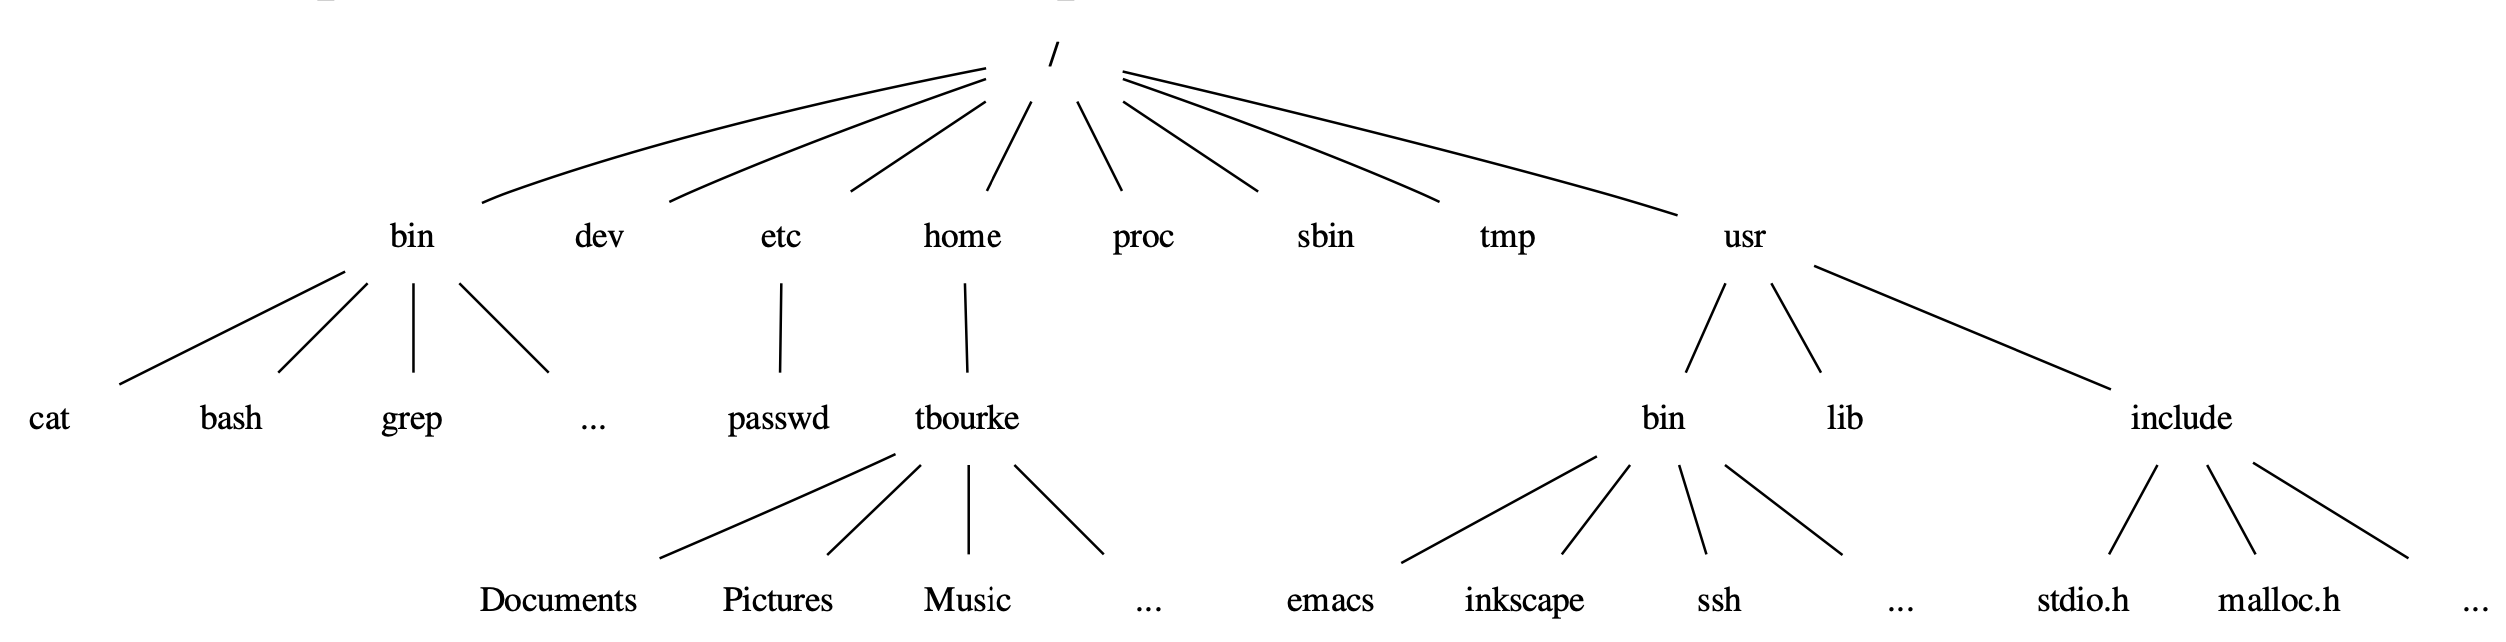
\includegraphics[scale=0.35]{unix-tree.png}
    \caption{Arborescence Unix par défaut}
\end{figure}

La commande \texttt{ls} utilisée avec un \emph{chemin relatif} permet d'afficher le contenu d'un dossier:
\begin{center}
    \texttt{ls /etc}
\end{center}

La commande \texttt{cat} permet d'afficher le contenu d'un fichier:
\begin{center}
    \texttt{cat /etc/passwd}
\end{center}

La commande \texttt{df} permet d'analyser comment le stockage physique est associé à la hiérarchie.

\paragraph{Standards} Cette hiérarchie suit des standards et conventions, qui sont détaillés dans le manuel \texttt{man hier}. On peut notamment citer:
\begin{itemize}
    \item \texttt{/bin}: les programmes utilisés pour les réparations, le démarrage, le mode à utilisateur unique
    \item \texttt{/sbin}: identique à \texttt{/bin}, mais n'est normalement pas exécuté par les utilisateurs normaux
    \item \texttt{/etc}: fichiers de configuration du système
    \item \texttt{/home}: dossiers des utilisateurs
    \item \texttt{/tmp}: fichiers temporaires, pouvant être nettoyé au redémarrage
    \item \texttt{/var/tmp}: fichiers temporaires conservés au redémarrage
    \item \texttt{/usr}: contient la majorité des programmes, bibliothèques
    \item \texttt{/dev}: fichiers spéciaux pour accéder aux appareils d'entrée et de sortie 
\end{itemize}

Les commandes suivantes sont utiles pour manipuler des fichiers et dossiers:
\begin{itemize}
    \item \texttt{mkdir} créé un nouveau dossier
    \item \texttt{rmdir} supprime un dossier vide
    \item \texttt{rm} supprime un fichier
    \item \texttt{find \emph{path}} affiche une sous-arborescence ou des fichiers qui vérifient le critère spécifié
\end{itemize}

\end{document}